\documentclass{article}
\usepackage[utf8]{inputenc}
\usepackage[english]{babel}

\textwidth 16.2cm \textheight 23cm \topmargin -0.6cm
\oddsidemargin 0.31cm \evensidemargin -0.91cm

\usepackage{amsmath}
\usepackage{amsfonts}
\usepackage{amsbsy}
\usepackage{amssymb}
\usepackage{graphicx}
\usepackage{psfrag}
\usepackage{epsfig}
\usepackage{multicol}
\usepackage{cite}
\usepackage{color}
\usepackage{dsfont}
\usepackage[center]{caption}
\usepackage{listings} 
\usepackage{xcolor} 
\usepackage{textcomp} 

\newcommand {\defeq}    {\stackrel{\rm def}{=}}

\DeclareMathOperator{\Span} {{Span}}
\DeclareMathOperator{\gap} {{gap}}
\DeclareMathOperator{\ddiv} {{div}}
\DeclareMathOperator{\argsup} {{argsup}}
\DeclareMathOperator{\argmin} {{argmin}}
\DeclareMathOperator{\dom} {{dom}}
\DeclareMathOperator{\epi} {{epi}}

\newtheorem{thm}{Theorem}
\newtheorem{prop}{Proposition}
\newtheorem{lemma}{Lemma}
\newtheorem{defn}{Definition}
\newtheorem{cor}{Corollary}
\newtheorem{model}{Model}
\newtheorem{rmk}{Remarque}
\newtheorem{ans}{Answer}
\newtheorem{ass}{Assumption}
\newtheorem{algo}{Algorithme}

\def\endproof{\hfill $\Box$\newline\newline}
\def\proof{\par\noindent{\it Proof}. \ignorespaces}

\title{Image Deblurring with Blurred/Noisy Image Pairs}
\author{Yohann Salaun}
\date{\today}

\parindent=0pt
\begin{document}
\maketitle

\section{Introduction}

Taking a picture under low light condition often results in bad quality images. With SLR camera, options as ISO, exposure time and aperture can be better chosen to fit the bad light conditions. However, even with such gears, the picture is not as perfect when taken with hands only. A noise/blur dilemma appears and it is often impossible to avoid at least one of these artifacts. The aim of \cite{deblur_denoise} is to mix up two pictures facing a strong noise for one and a strong blur for the other in order to create a picture that is nor blurry nor noisy.


\begin{figure}[ht]
\begin{center}\begin{tabular}{c}	
	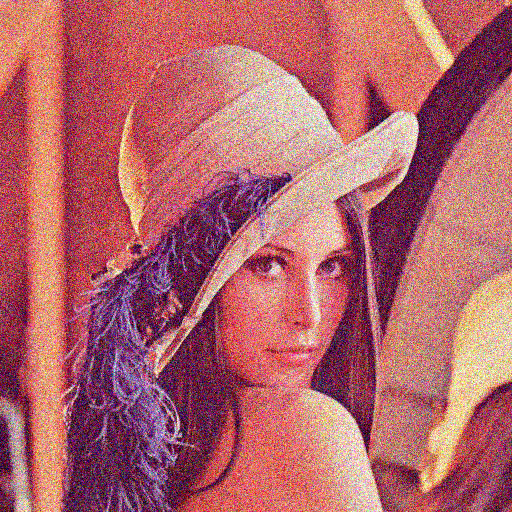
\includegraphics[scale=0.4]{images/lena_noisy.jpg}
	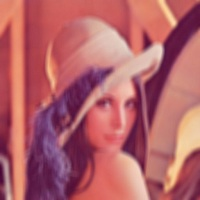
\includegraphics[scale=0.4]{images/lena_blurred.jpg}
\end{tabular}
	\caption{De gauche à droite, l'image originale, bruitée avec un bruit décart type 10 puis débruitée avec $\mu = 2$, $\epsilon = 10^{-4}$.}\label{surfplot}\end{center}
\end{figure}

\section{References}

\begin{thebibliography}{9}

\bibitem{deblur_denoise}
	L. Yuan, J. Sun, L. Quan, and H-Y. Shum
	\emph{Image Deblurring with Blurred/Noisy Image Pairs}.
	ACM SIGGRAPH,
	2007. 


\end{thebibliography}


\end{document}
